%==============================================================================
% Šablona prezentace/Presentation template
% Autoři / Authors: Zdeněk Vašíček, Aleš Smrčka, Jaroslav Dytrych, Jana Stopková, Kristýna Zaklová, Adam Herout
% Kontakt pro dotazy a připomínky: sablona@fit.vutbr.cz
% Contact for questions and comments: sablona@fit.vutbr.cz
%==============================================================================

\documentclass[]{fitthesispresn}
% Je-li prezentace v anglickém jazyce, je zapotřebí u třídy použít parametr english následovně (ev. zakomentovat předcházející řádek a odkomentovat následující): / If presentation is in English, it is necessary to use parameter english as follows (or comment the previous line and uncomment the following one):
%\documentclass[english]{fitthesispresn}

% Nastavení informací pro úvodní stránku / Setting information for the title page
%---------------------------------------------------------------------------
\projectinfo{
  date=\today, % Datum - je vhodné vepsat datum obhajoby (natvrdo), ne datum kompilace slajdů / Date - it is advisable to write the date of the defense (hard), not the date of the slide compilation        
  title={Emulátor herní konzole PlayStation 1 s vyšším renderovacím rozlišením}, % Název prezentace / Presentation title (The whole title of the presented work suitably divided into lines that are optically balanced)
  title.footer={PlayStation 1 emulátor}, % Název prezentace - text zobrazovaný vedle čísla slajdu / Presentation title - displayed next to the slide number (The full title of the presented work, it may be suitably abbreviated to fit the footer)
  author.name={Filip},  % Jméno autora / Author name
  author.surname={Stupka}, % Příjmení autora / Author surname
  author.title.first={Bc.}, % Tituly před jménem autora (jsou-li jaké) / Author's titles before the name (if there are any)
  supervisor.name={Jiří}, % Jméno vedoucího / Supervisor name
  supervisor.surname={Jaroš}, % Příjmení vedoucího / Supervisor surname
  supervisor.title.first={doc. Ing.}, % Tituly před jménem / Supervisor's titles before the name
  supervisor.title.last={Ph.D.} % Tituly za jménem / Supervisor's titles after the name
}

% Struktura prezentace / Presentation structure
%---------------------------------------------------------------------------

\begin{document}
    \frame[plain]{\titlepage} % Úvodní stránka / Title page
    \ifczech
        %%%%%%%%                        01 - Motivace                       %%%%%%%%
%---------------------------------------------------------------------------
% Při prezentování nejvíc záleží na začátku. 
% Pro získání pozornosti na začátku veřejné řeči se doporučuje: říct nějakou statistiku; položit otázku (u státnic spíše řečnickou).

% HEROUT, Adam. Prezentování. Herout.net: Poznámky učitele, kouče, čtenáře. [online]. [cit. 2021-9-15]. Dostupné z: https://www.herout.net/blog/category/prezentovani/
%---------------------------------------------------------------------------

% - Uveďte posluchače do tématu své práce.
% - Řekněte něco málo o stavu před zahájením práce a jaké byly důvody pro její vypracování.
% - Nejlepší je vysvětlit motivaci pomocí schématu. Pokud musíte použít odrážky, tak super-stručné, abyste je nečetli, ale ony pouze tvořily kostru sdělení.

% Z této části prezentace musí posluchači dostat stručné a výstižné odpovědi na otázky:
%  A) Proč děláte, co děláte? K čemu je to dobré?
%  B) Co je cílem práce? Co má být výsledkem?

% Odolejte pokušení říkat banality a všeobecně známé informace.
% "Žijeme v době rozvoje mobilní výpočetní techniky, kdy každý má v kapse mobil" - je dokonale prázdné a hloupé sdělení, nic takového neříkejte, fakt to nikoho nezajímá.

\begin{frame}
  \frametitle{Motivace}
  \begin{columns}
    \column{0.4\textwidth}
    \begin{itemize}
        \item Historické hry
        \item \emph{87\%} nedostupných
        \item \emph{Legalita} získání her
        \item Nedostupný \emph{harware}
    \end{itemize}
     
    \column{0.6\textwidth}
    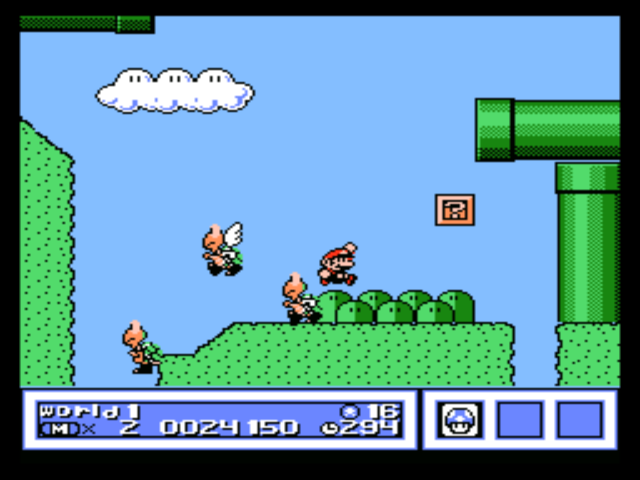
\includegraphics[width=\textwidth]{img/smb3.png}
  \end{columns}
\end{frame}


%%%%%%%%                       02 - Cíle práce                      %%%%%%%%
%---------------------------------------------------------------------------
% Stručně uveďte cíle Vaší práce.
% Vhodné jsou max. 3 odrážky/věty s hlavními cíli.

% Někdy je motivace totožná s formulací cílů. Nenuťte se do dvou slajdů, když je správnější myšlenku vyjádřit jedním... 

% Formulujte, co je cílem:
%  - Jak se pozná úspěšný výsledek?
%  - Co jsou výstupy?
%  - Jaké vlastnosti má mít úspěšný výsledek?
%  - Kde to půjde použít?

% Lepší je bez použití odrážek:
%  - mít dostatečně dobrý obrázek, který budete svými slovy komentovat 
%  - na obrázku je vizuální sdělení, sdělení slovní dodáte pusou

% Je zbytečné říkat generická a obecná tvrzení: "Řešení by mělo být rychlé, spolehlivé a robustní" - toto jsou obecné požadavky na cokoli a informační hodnota sdělení je NULA - je to jen plýtvání časem a inteligencí.
% Mluvte konkrétně: Jaké konkrétní vlastnosti má mít Vaše řešení, co konkrétně znamená "robustní", co konkrétně znamená "spolehlivé"?

\begin{frame}
  \frametitle{Cíle práce}
  \begin{columns}
    \column{0.3\textwidth}
    \begin{itemize}
        \item \emph{PlayStation 1} emulátor
        \item \emph{Změna} rozlišení
        \item Použitelnost
        \item Ovládání
    \end{itemize}
     
    \column{0.7\textwidth}
        
\includegraphics[width=\textwidth]{img/dolphin-resolution.jpg}
  \end{columns}
\end{frame}


%%%%%%%%                  03 - Informace o řešení                   %%%%%%%%
%---------------------------------------------------------------------------
% Cílem  obhajoby je podat zprávu o stavu projektu, nikoliv tedy držet přednášku na zadané téma. Mluvte o tom, co vy jste udělali, jaké jsou vaše výsledky. Mějte na slajdech formální pojmy, buďte přesní, definujte a odkazujte se.

% Prezentace nemusí a vlastně nemá obsahovat:
% -- Výklad použitých algoritmů apod. To patří do přednášky na dané téma, v prezentaci o stavu jen známé algoritmy uveďte podle jména, neznámé algoritmy třeba trochu přibližte, aby bylo zřejmo, o co jde, ale nevysvětlujte je podrobně. Není cílem, aby vaši posluchači algoritmu rozuměli a dokázali ho naprogramovat, ale aby měli představu, na čem pracujete a jak se vám to daří.
% -- Podrobnosti návrhu vašeho systému. Opět, posluchači nebudou váš systém hackovat, nepotřebují detailní strukturu tříd, názvy funkcí, jména souborů, datové formáty apod. Tyto věci uvádějte pouze v takové míře, která pomůže posluchačům udělat si představu, na čem pracujete a jak se vám to daří.

% HEROUT, Adam. Prezentování. Herout.net: Poznámky učitele, kouče, čtenáře. [online]. [cit. 2021-9-15]. Dostupné z: https://www.herout.net/blog/category/prezentovani/
%---------------------------------------------------------------------------

% - Uveďte, jaké zajímavé problémy jste v práci řešili.
% - Mělo by z toho být patrné, že je to závěrečná práce -- ne jen další projekt do předmětu -- tedy je v tom něco netriviálního, zajímavého a přínosného.
% - Raději dva nebo tři slajdy, které ukážete/vysvětlíte během 20 vteřin, než se snažit všechno "namastit" na jeden slajd.
% - Na slajdy je dobré dát vizuální informaci: vzorce, schemata, obrázky, diagramy. Slovní informaci můžete předat pusou. Je dokonale zbytečné a otravné mít na slajdu v odrážkách to samé, co se chystáte říct.
% - Titulek slajdu "Podstatné informace o řešení" je hodně generický. Ve skutečné Vaší prezentaci bude daleko lepší použít specifický titulek na každém ze slajdů, například: "Schéma neuronové sítě pro detekci frňáků", "Návrh nekonečného automatu", "Vytvořená datová sada" apod.

\begin{frame}
  \frametitle{Architektura}
  \begin{columns}
    \column{0.3\textwidth}
    \begin{itemize}
      \item CPU
      \item GPU
      \item SPU
      \item MDEC
      \item CD-ROM
    \end{itemize}
    \column{0.7\textwidth}
      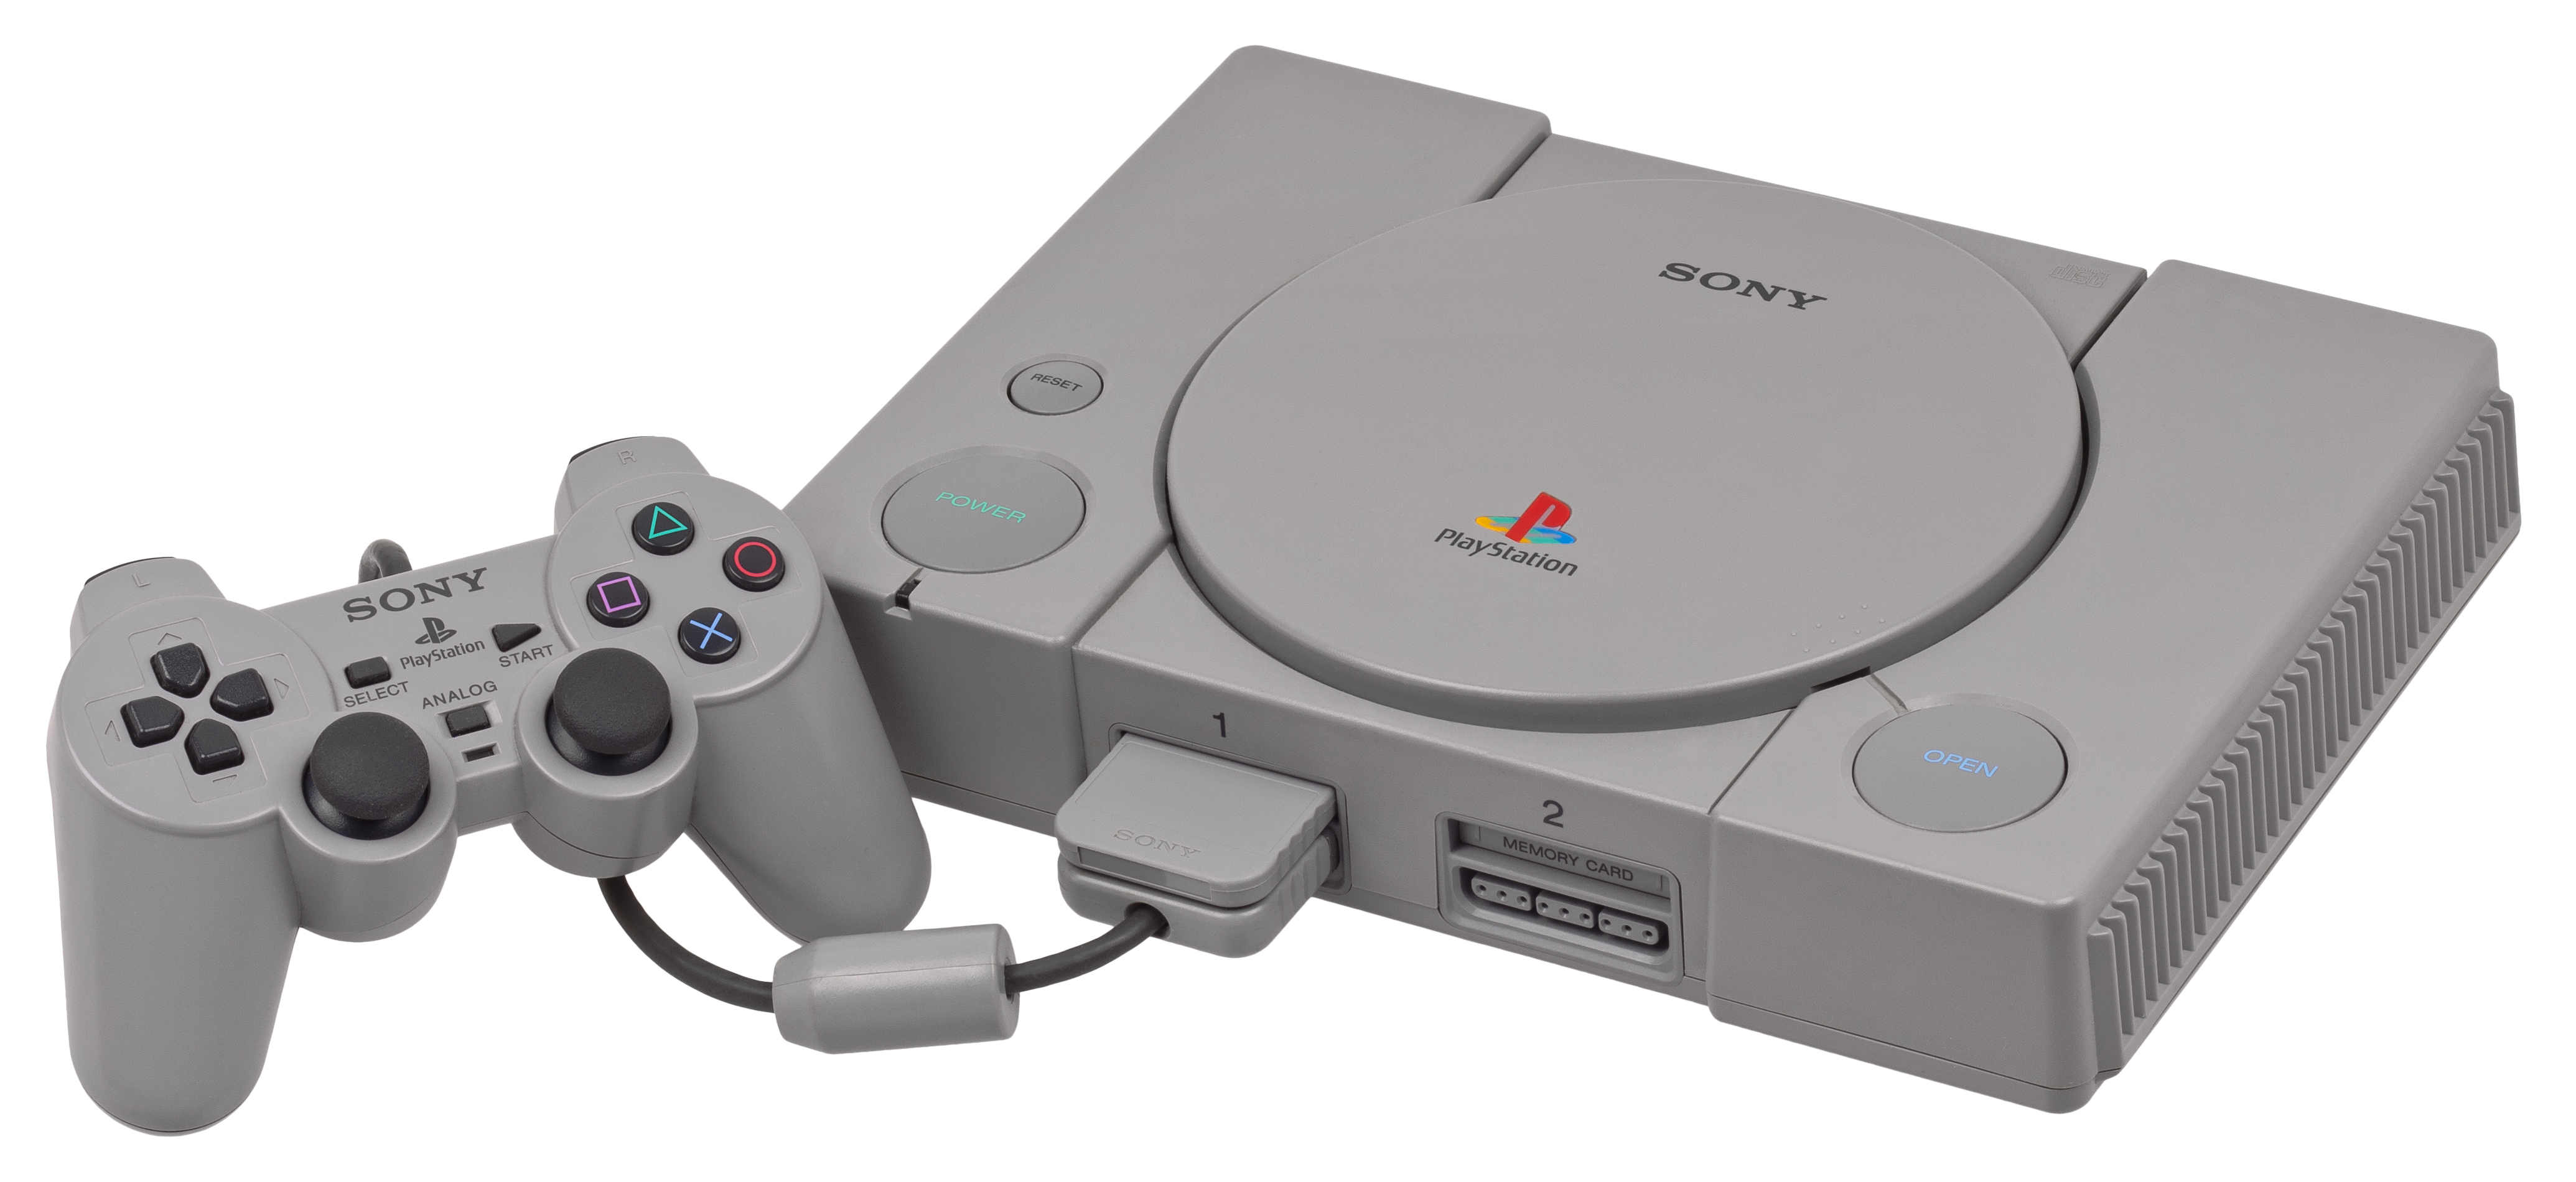
\includegraphics[width=\textwidth]{img/psx-console.jpg}
  \end{columns}
\end{frame}

\begin{frame}\frametitle{Architektura}
  \makebox[\linewidth]{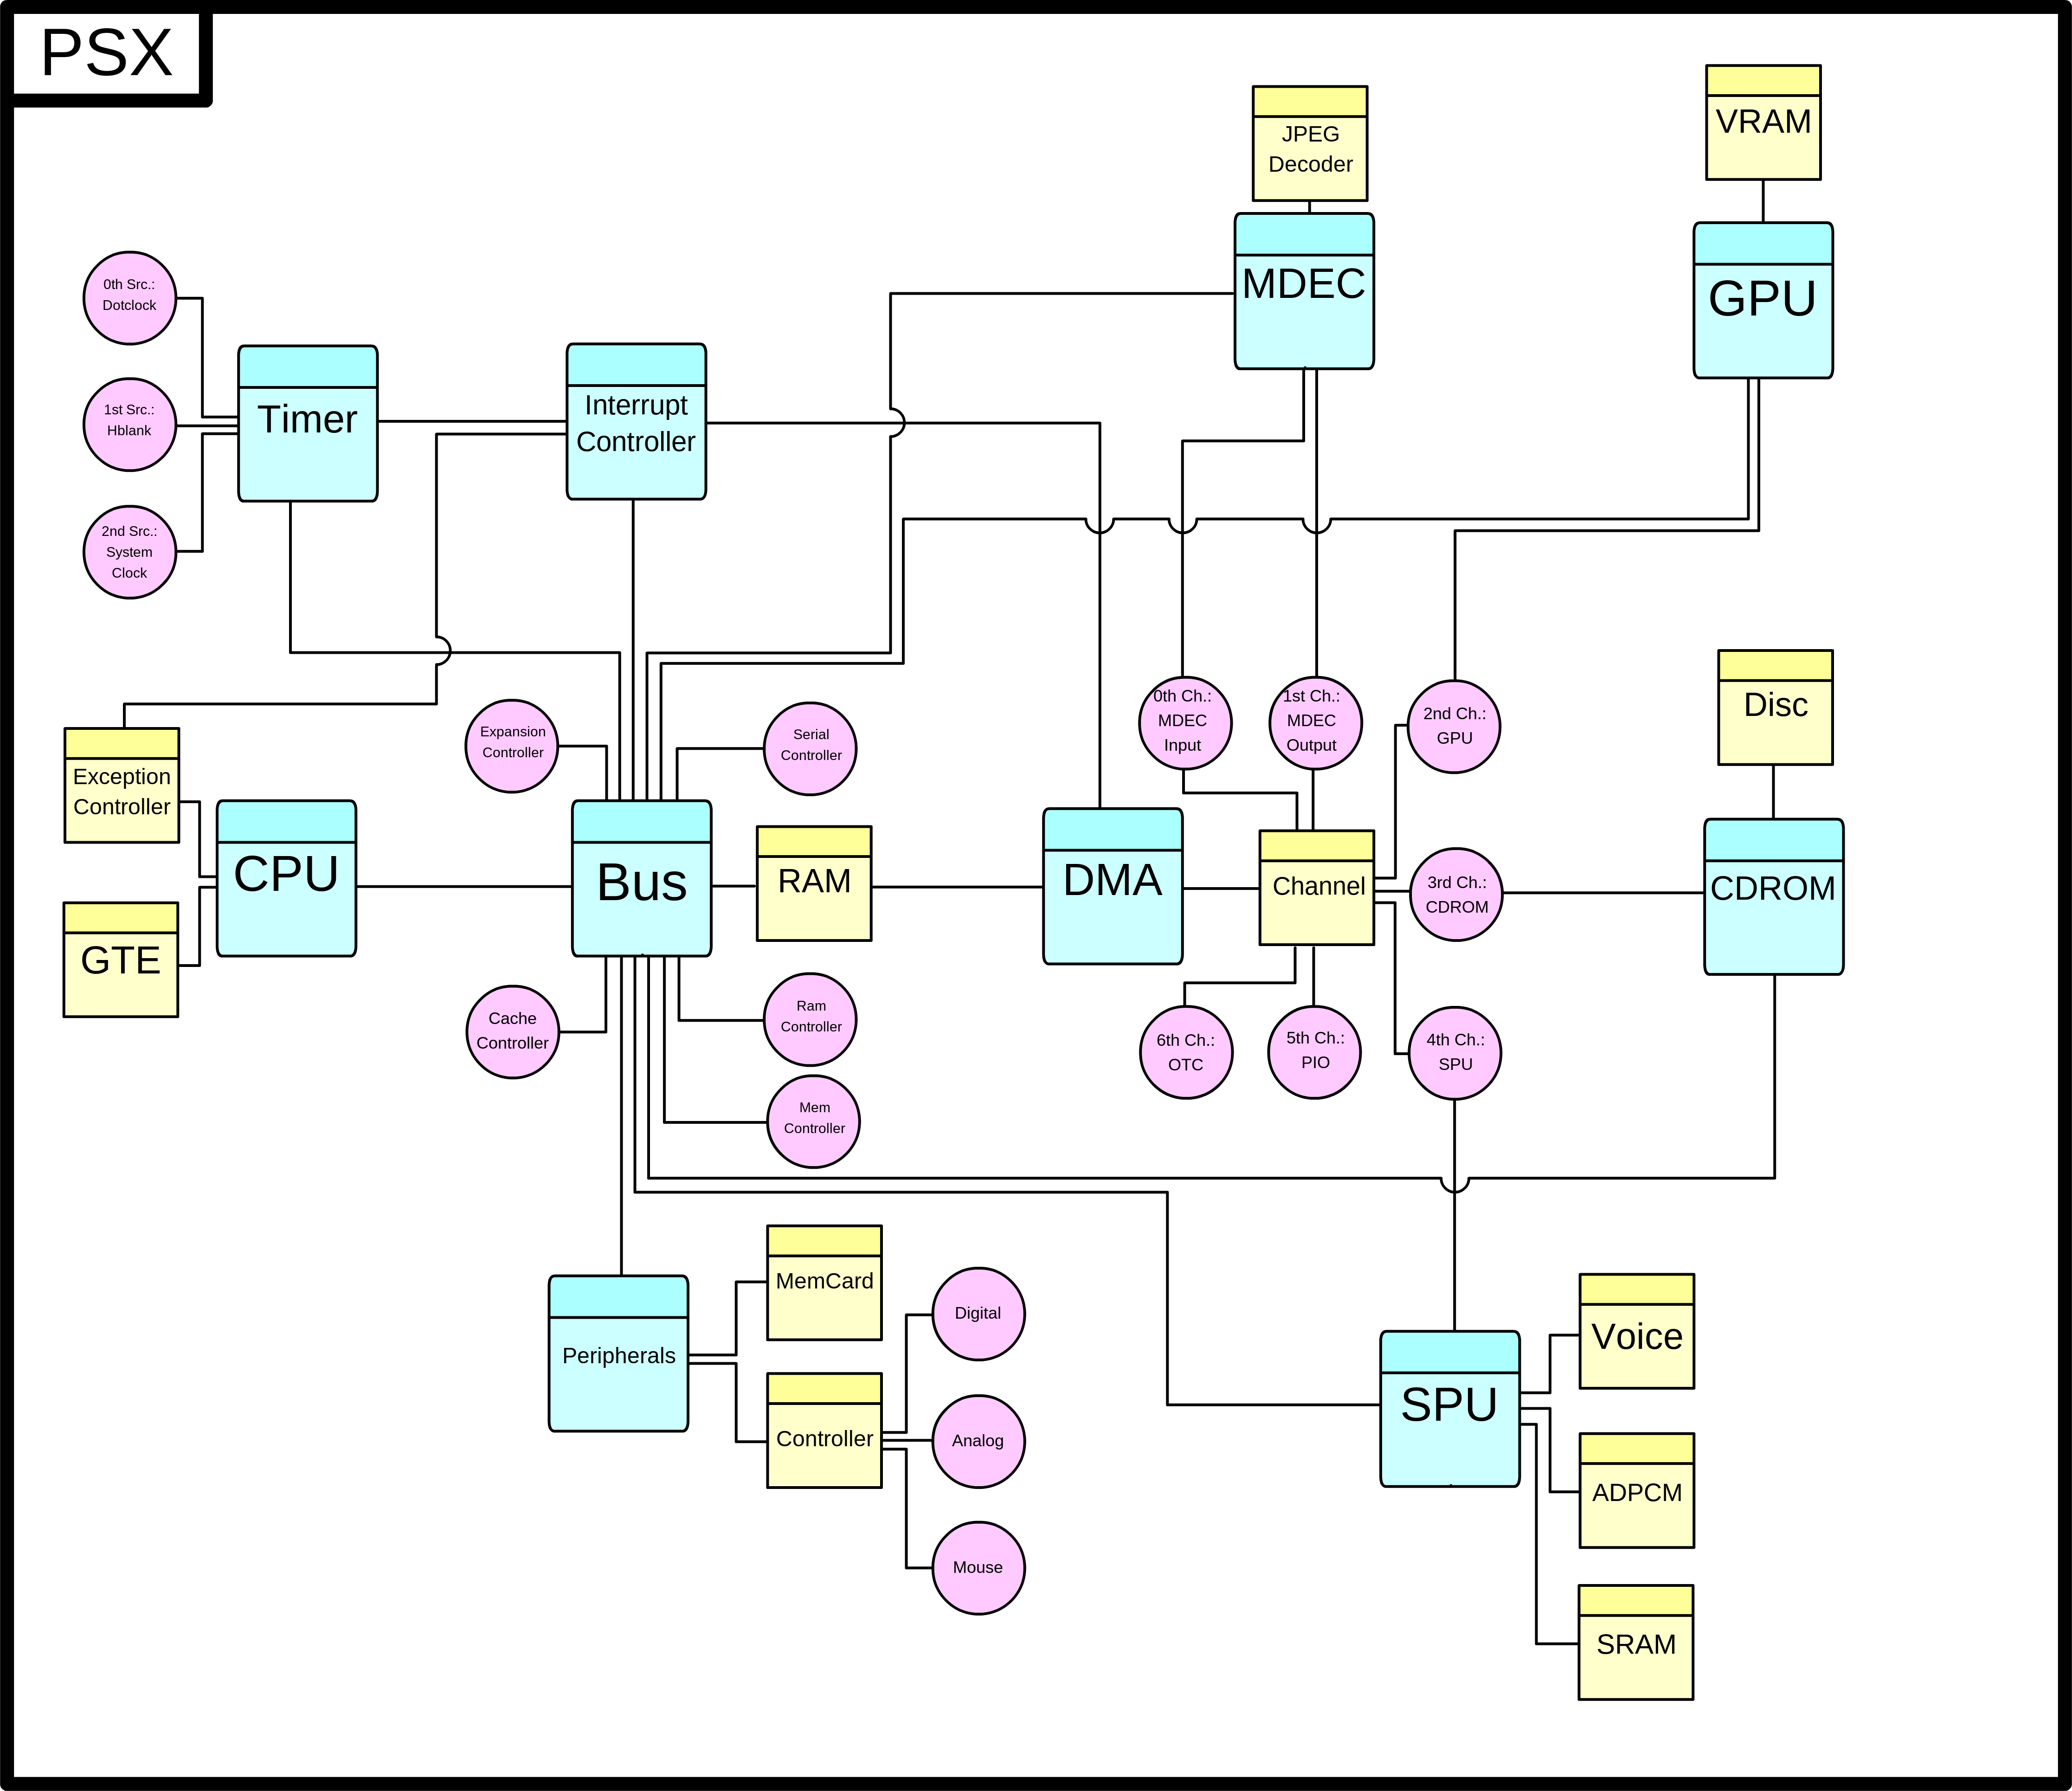
\includegraphics[width=0.7\paperwidth]{img/psx-layout.png}}
\end{frame}


%%%%%%%%                    04 - Výsledky práce                     %%%%%%%%
%---------------------------------------------------------------------------
% Shrňte, jakých výsledků se Vám podařilo dosáhnout.
% Uveďte, jakým způsobem byla vyhodnocena funkčnost a správnost řešení.
% Buďte konkrétní: místo "Aplikace je otestovaná", řekněte, kým a jak byla testována, jaké byly výsledky testů.
% Místo "Úspěšnost detektoru je hodně dobrá" řekněte "Úspěšnost detektoru je 93 % mAP" nebo ještě radši ukažte tabulku se srovnáním oproti alternativním řešením.
% Pokud vyhodnocení sestávalo ze dvou nebo tří částí, může být vhodné rozdělit obsah na dva či tři slajdy. Při prezentování je ovšem potřeba se pohlídat, aby čas věnovaný každému slajdu byl adekvátně krátký a nedošlo k přetažení času.

\begin{frame}
  \frametitle{Výsledky práce}
  \begin{columns}
  \column{0.4\textwidth}
    Kompatibilita:
    \begin{itemize}
      \item \emph{1/8} z testovaných her \emph{dokončitelných}
      \item \emph{4/8} z testovaných her \emph{hratelných}
      \item \emph{3/8} z testovaných her \emph{nenastarovatelných}
    \end{itemize}
    Rychlost:
    \begin{itemize}
      \item 10 let starý laptop \emph{94\%-104\%}
      \item moderní počítač \emph{250\%-300\%}
    \end{itemize}
  \column{0.6\textwidth}
    \centering
    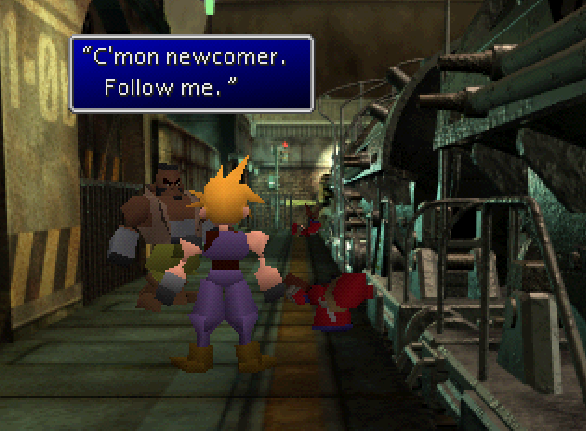
\includegraphics[width=0.7\textwidth]{img/ff7-showcase-1-1.png}
    
    \bigskip
    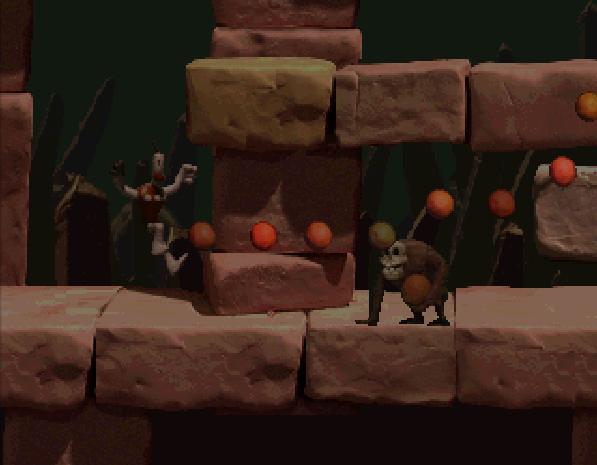
\includegraphics[width=0.7\textwidth]{img/skullmonkeys-showcase-1-1.png}
    
  \end{columns}
\end{frame}

\begin{frame}
  \frametitle{Výsledky práce}
  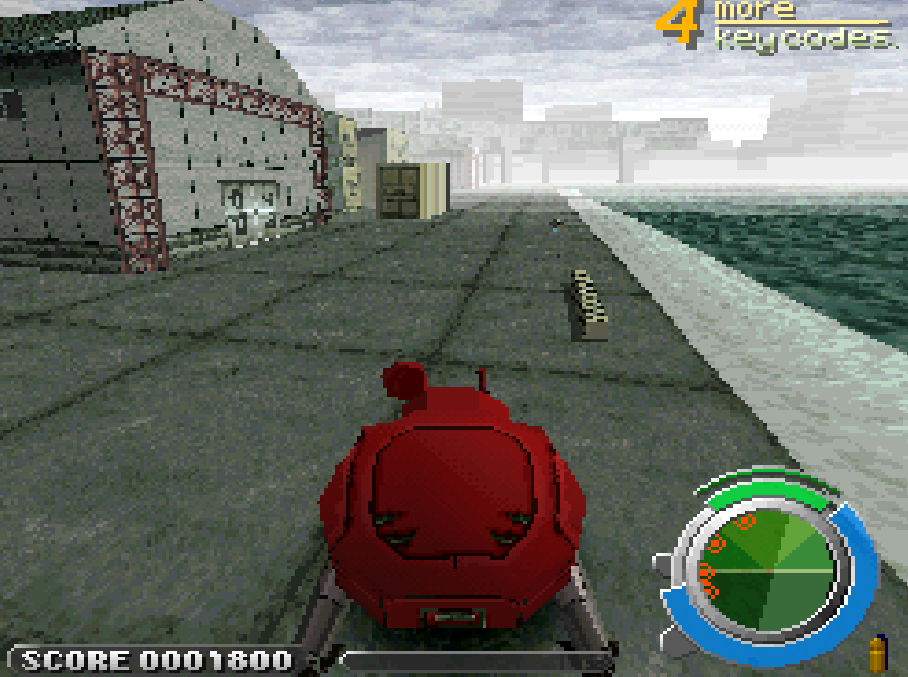
\includegraphics[width=1\textwidth]{img/gits-lowres.png}
\end{frame}

\begin{frame}
  \frametitle{Výsledky práce}
  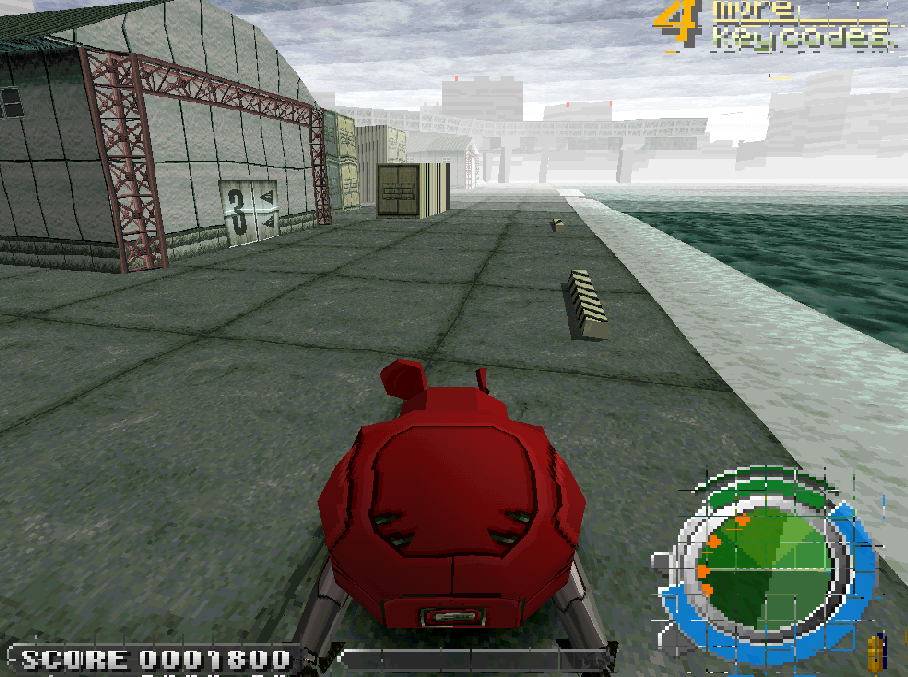
\includegraphics[width=1\textwidth]{img/gits-highres.png}
\end{frame}

\begin{frame}
  \frametitle{Výsledky práce}
  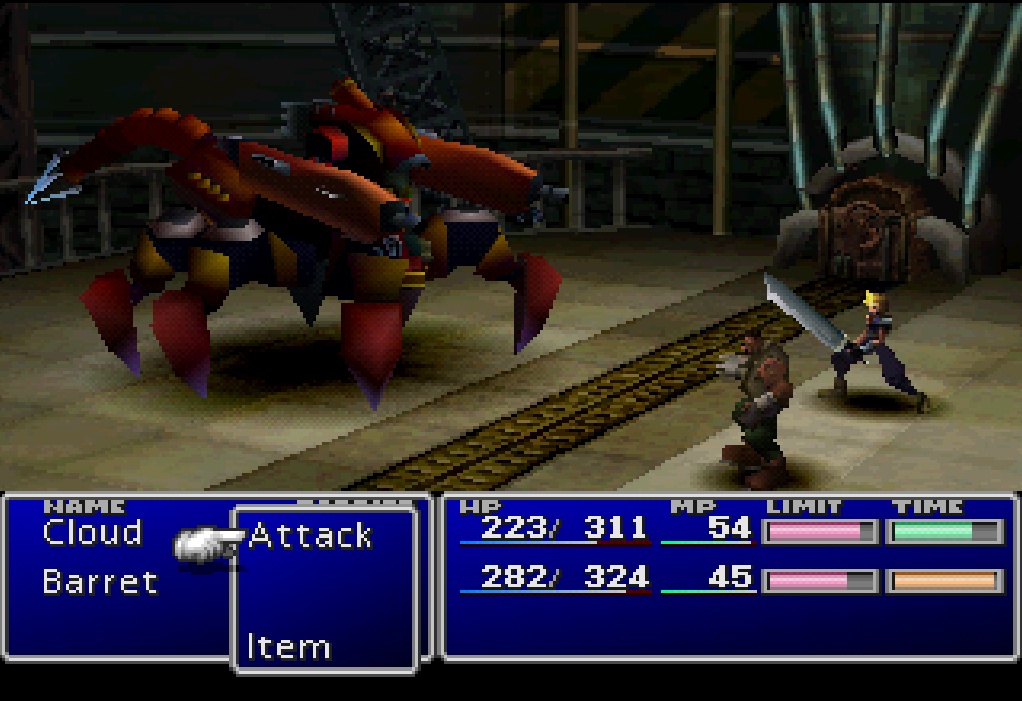
\includegraphics[width=1\textwidth]{img/ff7-lowres.png}
\end{frame}

\begin{frame}
  \frametitle{Výsledky práce}
  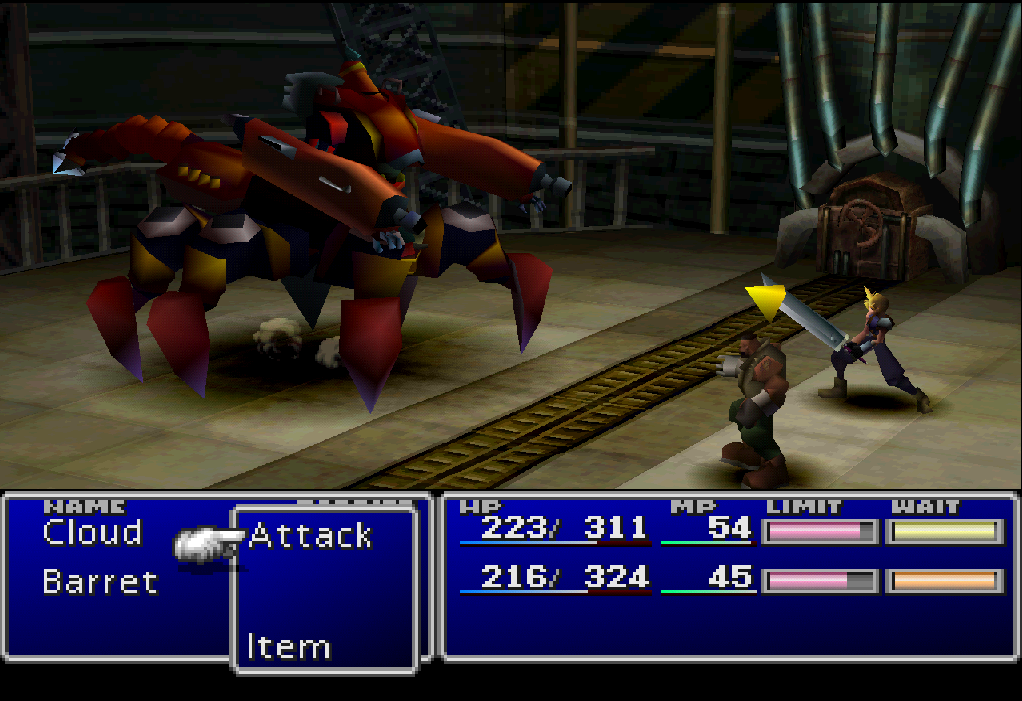
\includegraphics[width=1\textwidth]{img/ff7-highres.png}
\end{frame}

\begin{frame}
  \frametitle{Výsledky práce}
  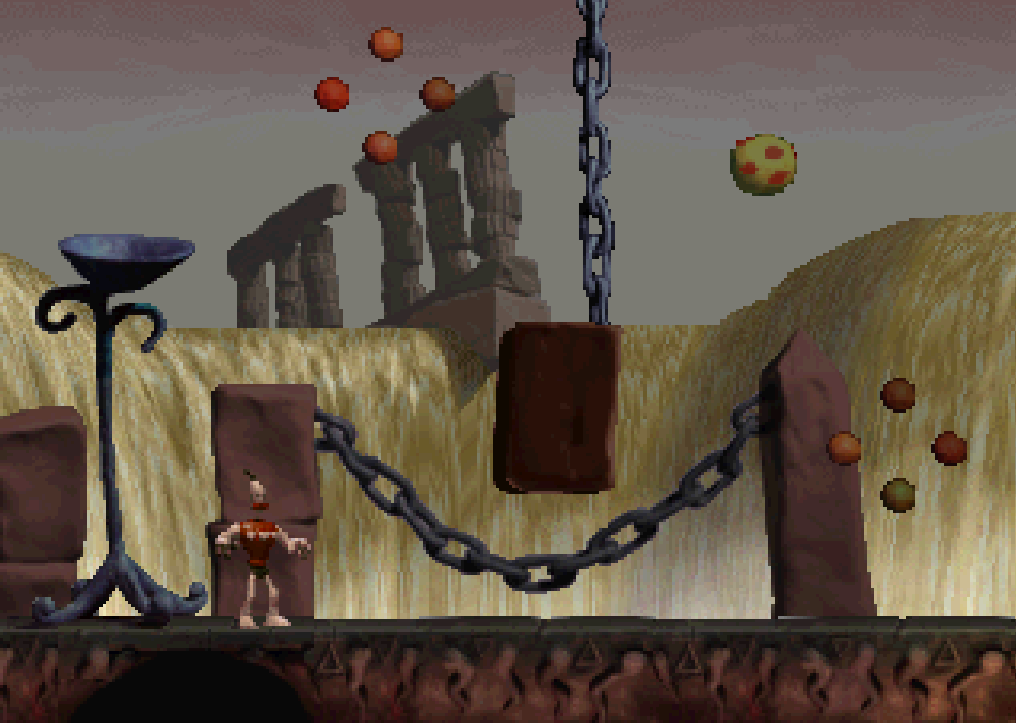
\includegraphics[width=1\textwidth]{img/skull-lowres.png}
\end{frame}

\begin{frame}
  \frametitle{Výsledky práce}
  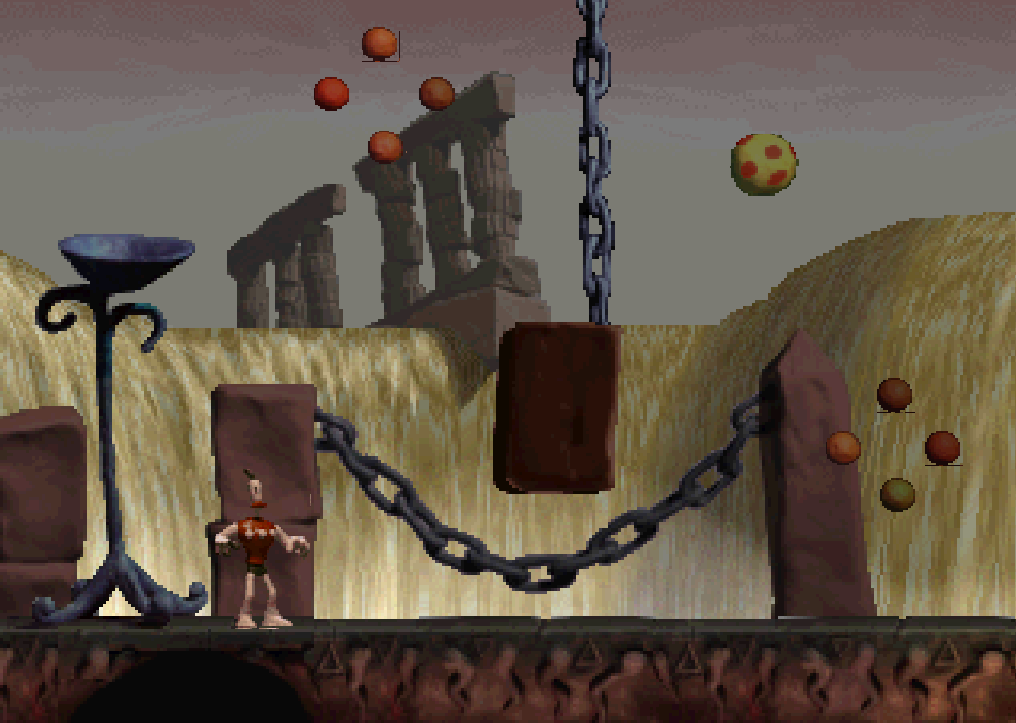
\includegraphics[width=1\textwidth]{img/skull-highres.png}
\end{frame}

%%%%%%%%                      05 - Poděkování                       %%%%%%%%
%---------------------------------------------------------------------------
% Na tomto slajdu by měl být buď jeden velký, nebo více menších vhodně poskládaných obrázků.
% Vyberte to nejlepší, čím se chcete pochlubit - komise se na tento slajd bude dívat nejdéle ze všech slajdů.
% U tohoto slajdu ústně poděkujete za pozornost (ne nutně textem přes celý slajd) a komise pak bude mít prostor pro jeho prohlížení při čtení posudků.
%---------------------------------------------------------------------------

% Co padne na konci prezentace, je to, co posluchači budou brát v úvahu při následném rozhodování.

% HEROUT, Adam. Prezentování. Herout.net: Poznámky učitele, kouče, čtenáře. [online]. [cit. 2021-9-15]. Dostupné z: https://www.herout.net/blog/category/prezentovani/
%---------------------------------------------------------------------------

\begin{frame}
  \frametitle{Děkuji za pozornost!}
  \centering
  \makebox[\textwidth]{
    \begin{tikzpicture}
      \node (screenshot) 
         {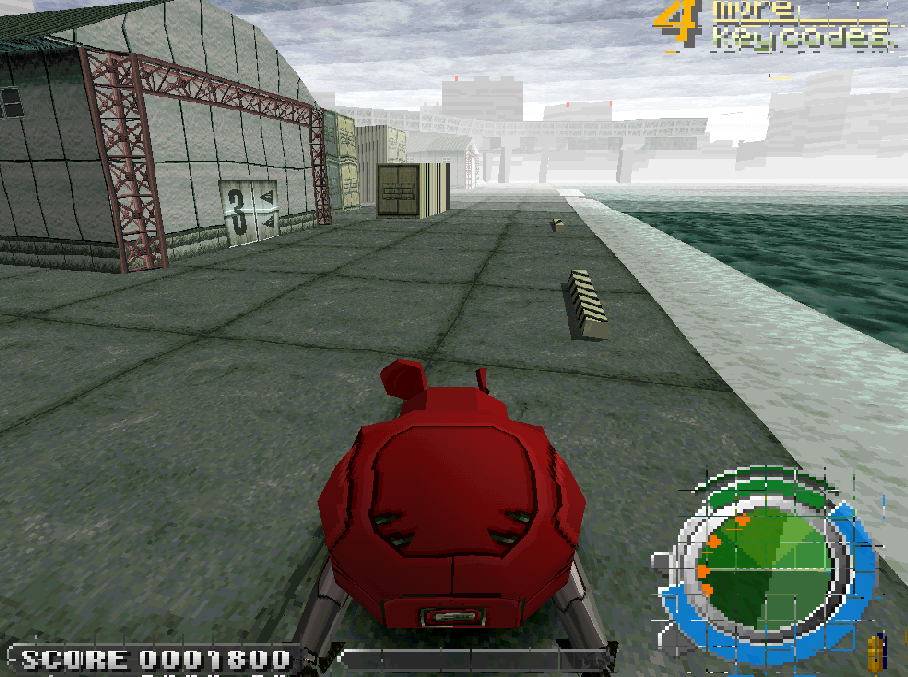
\includegraphics[width=0.5\paperwidth]{img/gits-highres.png}};
      \node (schema) at (screenshot.south east) [xshift=5em] [yshift=2.5ex]
         {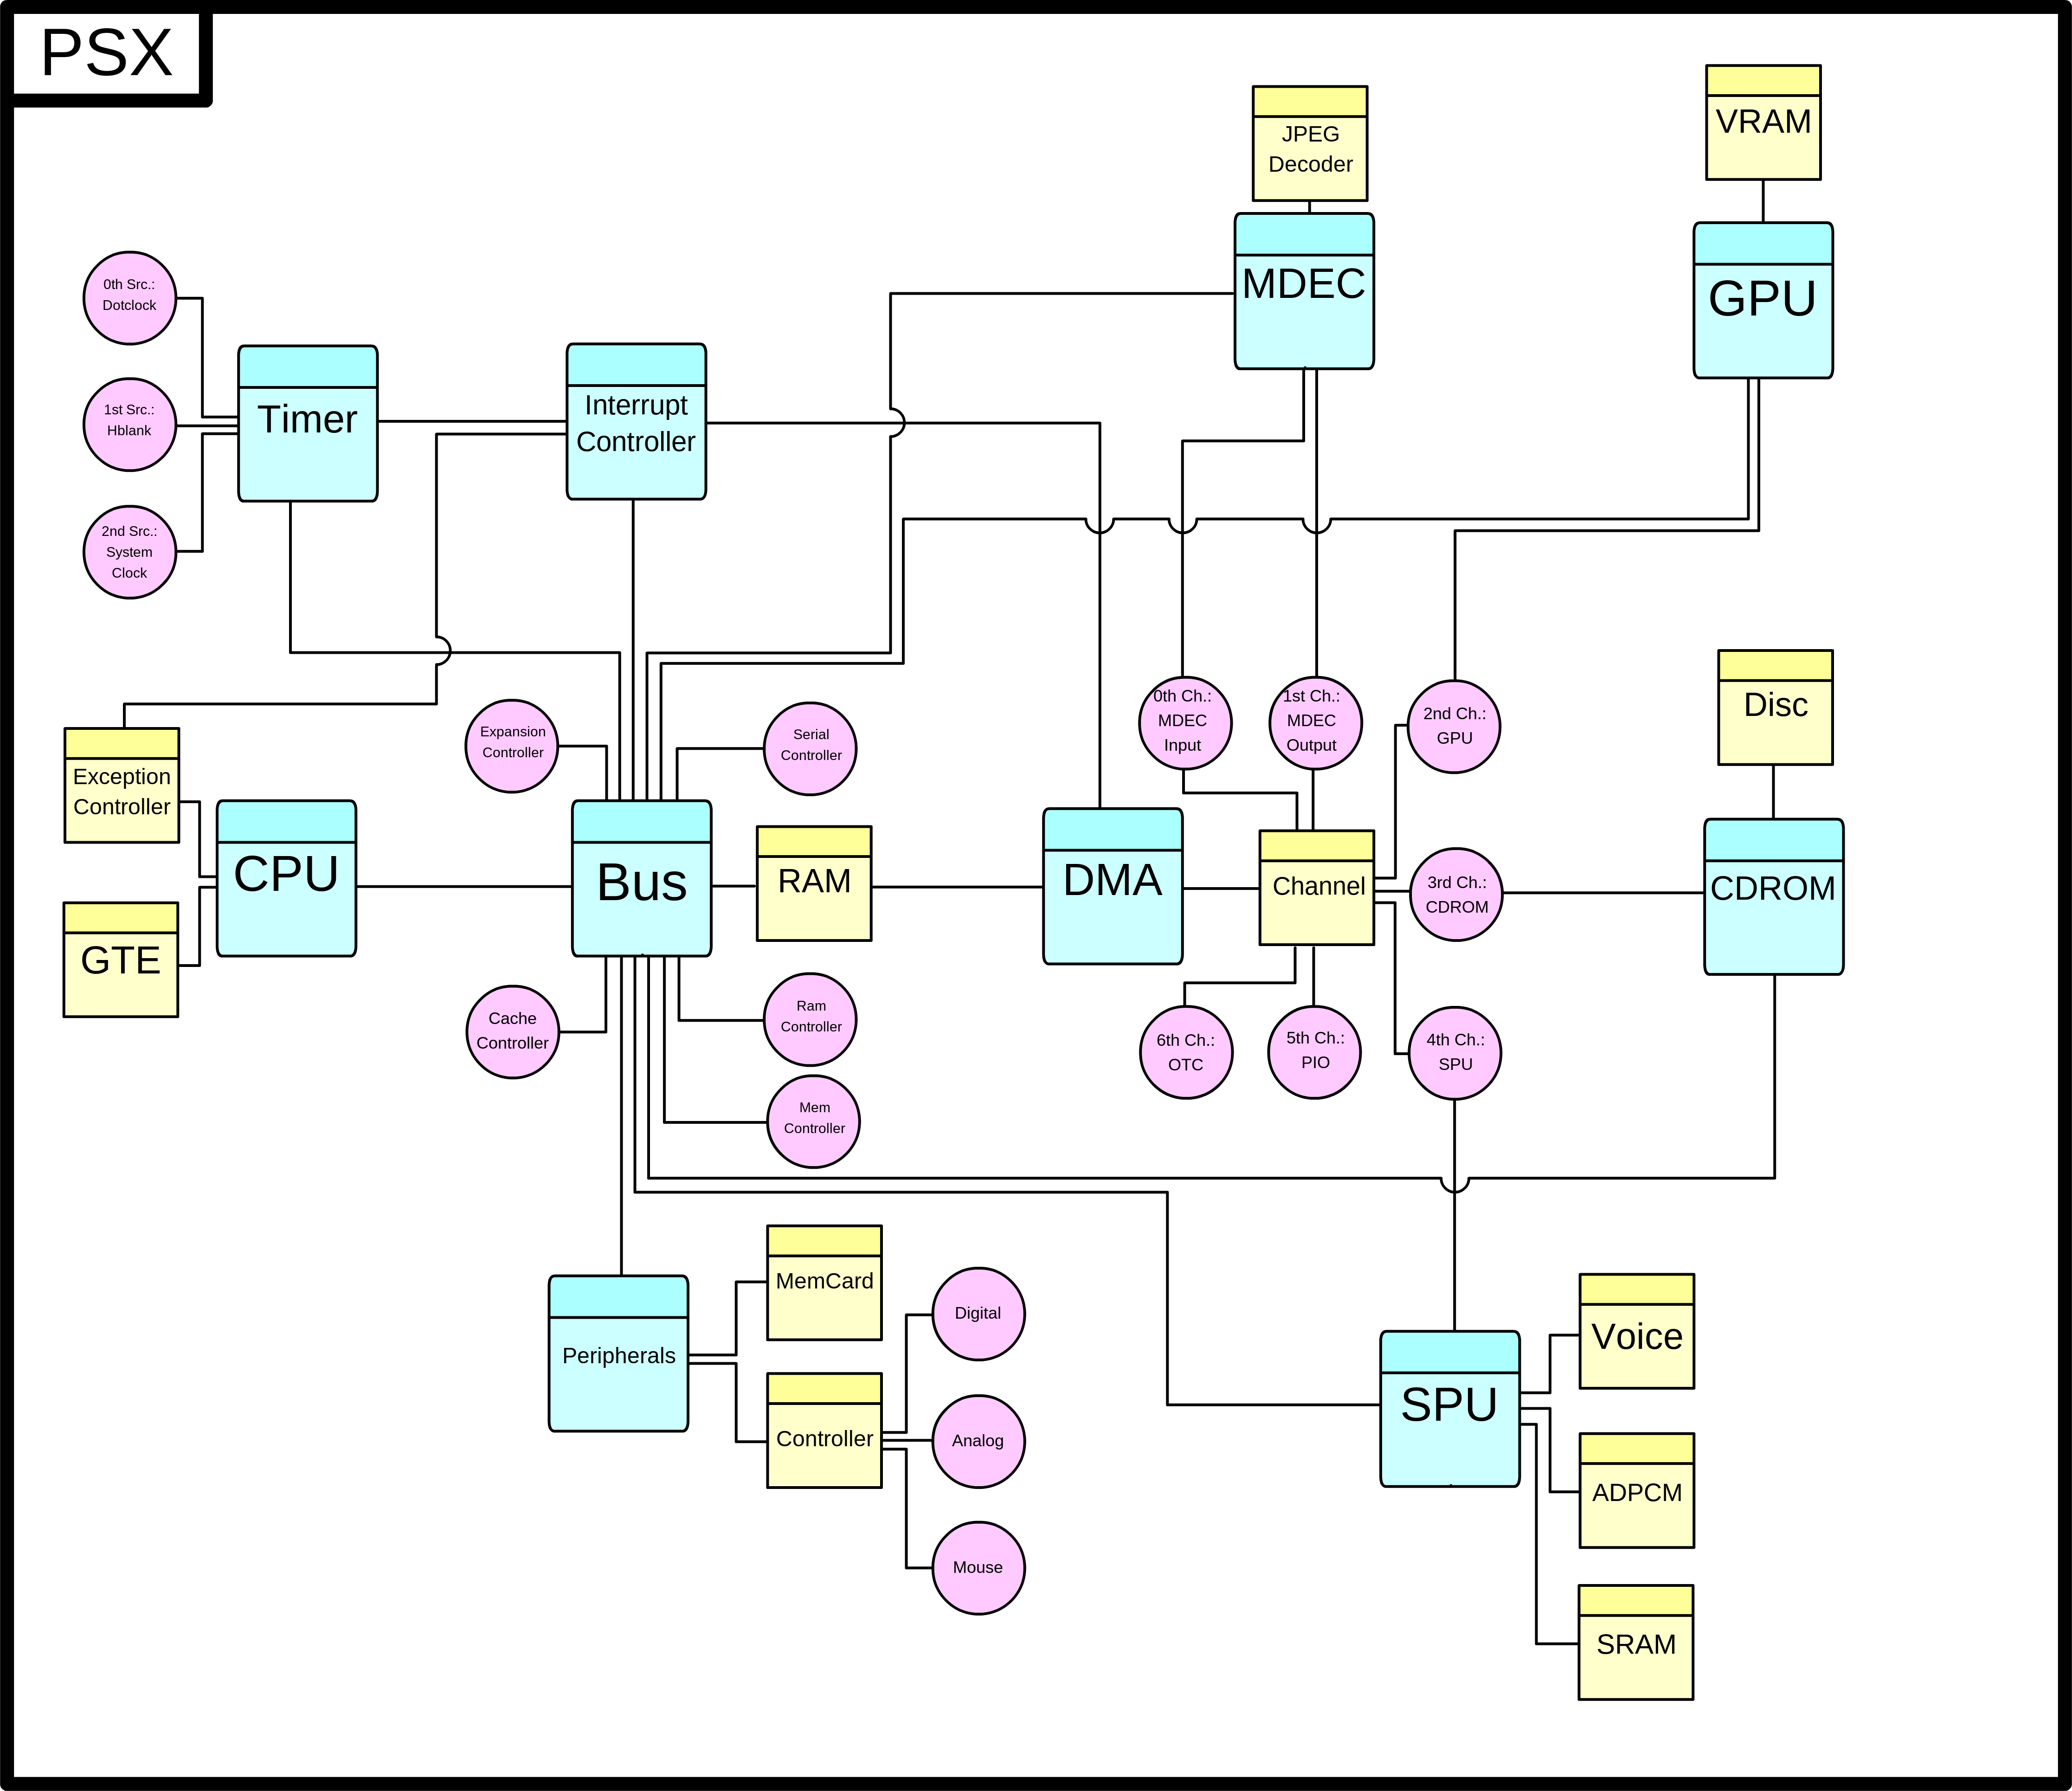
\includegraphics[width=0.30\paperwidth]{img/psx-layout.png}};
      \node (goal) at (screenshot.north east) [xshift=4em] [yshift=2ex]
         {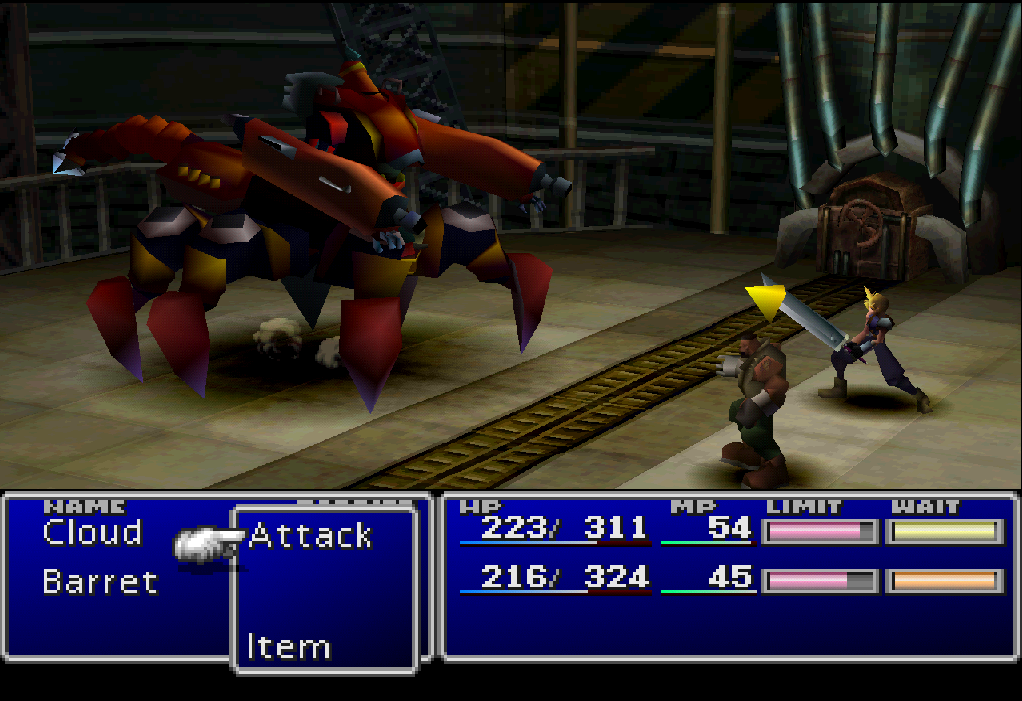
\includegraphics[width=0.4\paperwidth]{img/ff7-highres.png}};
    \end{tikzpicture}
  }
\end{frame}


%%%%%%%%                        06 - Otázky                         %%%%%%%%
%---------------------------------------------------------------------------
% U státnic student:
%   1) Prezentuje o své práci, skončí "Děkuji za pozornost!"
%   2) Předseda komise organizuje, co bude dál: čte se výtah z posudků.
%   3) Student zodpoví otázky, které oponent napsal do svého posudku.
%   4) Student odpovídá na otázky, které padnou v místnosti: od členů komise, ale třeba i od hostů.

% Pro bod 3) výše je vhodné mít připravené slajdy, které v odpovídání pomůžou:
%   A) Ukážou doslovný text otázky oponenta, student ji přečte, aby ji všichni znali, a pak na ni odpoví.
%   B) Budou obsahovat vizuální pomůcky k odpovědi.
%       a) Některé odpovědi na otázky žádnou vizuální pomůcku nepotřebují: student prostě řekne odpověď a všechno je jasné.
%       b) U jiných odpovědí je rozumné mít připravený obrázek, tabulku, graf, cosi, na čem odpověď jasně ukáže.

% Otázky oponenta nebývají myšlené jako "témata na přednášku". Pokud je možné odpovědět jednou větou, je to lepší, než mlžit okolo.
% Vizuální pomůcky často pomáhají ke stručné odpovědi: "Na schématu je vidět, že problém X řeším takto." A hotovo...

% Pokud k otázkám nebude potřeba žádná vizuální informace, je vhodné mít jednotlivé otázky jako odrážky na jediném slajdu.
% Pokud je otázek více a jsou k nim obrázky či grafy, je vhodné mít pro každou otázku jeden slajd - nahoře znění otázky, pod ním vizuální materiál.

\begin{frame}
  \frametitle{Dotazy}
  \begin{itemize}
    \item "Můžete ve stručnosti zmínit, zda existují kromě vašeho řešení ještě nějaké další softwarové nástroje pro simulaci chování herní konzole PS1 a tyto případně s vaším řešením porovnat?"
  \end{itemize}
\end{frame}

\begin{frame}
  \frametitle{Dotazy}
  \begin{center}
  \begin{tabular}{|c|c|c|}
      \hline
       & \textbf{PSX ReARMed} & \textbf{Restation} \\
      \textbf{JIT} & \color{green}ANO & \color{red}NE \\
      \textbf{SaveState} & \color{green}ANO & \color{green}ANO \\
      \textbf{HW Rasterizace} & \color{green}ANO & \color{red}NE \\
      \textbf{Změna rozlišení} & \color{red}NE & \color{green}ANO \\
      \textbf{HLBIOS} & \color{green}ANO & \color{red}NE \\
      \hline
  \end{tabular}
  \end{center}
\end{frame}

\begin{frame}
  \frametitle{Dotazy}
  \begin{itemize}
    \item "Co konkrétně by bylo třeba doimplementovat pro zlepšení synchronizace mezi komponentami při DMA přenosech?"
  \end{itemize}
\end{frame}
  % Slajdy v češtině / Slides in Czech
    \else
        %%%%%%%%                       01 - Motivation                      %%%%%%%%
%---------------------------------------------------------------------------
% When presenting, the beginning is what matters most. 
% To attract attention at the beginning of a public speech, it is advisable to: tell a statistic; ask a question (more like a rhetorical question for the state final exam).

% HEROUT, Adam. Prezentování. Herout.net: Poznámky učitele, kouče, čtenáře. [online]. [cit. 2021-9-15]. Available at: https://www.herout.net/blog/category/prezentovani/
%---------------------------------------------------------------------------

% - Introduce the audience to the topic of your thesis.
% - Tell a little about the situation before you started your work and what were the reasons for developing it.
% - It is best to explain the motivation using a scheme. If you must use bullet points, make them super-short so you don't read them, but they only form the skeleton of the message.

% From this part of the presentation, the audience must get brief and concise answers to the questions:
%  A) Why your work should matter? What is it good for?
%  B) What is the aim of the work? What should be the result?

% Resist the temptation to say banalities and common knowledge.
% "We live in an age of mobile computing where everyone has a mobile phone in their pocket" - is an empty and stupid statement, don't say anything like that, nobody cares.

\begin{frame}
  \frametitle{Motivation}
  \begin{columns}
    \column{0.4\textwidth}
    \begin{itemize}
        \item \emph{Inputs} or state \emph{before}
        \item What should be the~\emph{outputs}
        \item \emph{No} or \emph{brief} bullets!
        \item Desirable: A scheme with inputs and outputs
    \end{itemize}
     
    \column{0.6\textwidth}
    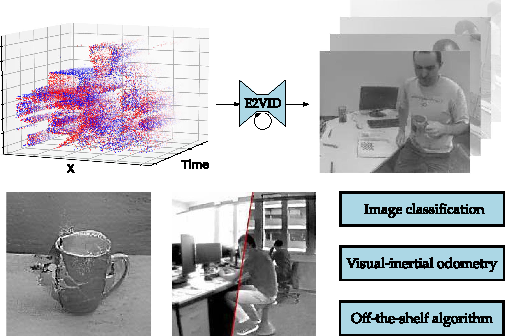
\includegraphics[width=\textwidth]{img/template-Teaser.pdf}
  \end{columns}
\end{frame}


%%%%%%%%                       02 - Objectives                      %%%%%%%%
%---------------------------------------------------------------------------
% Briefly state the objectives of your thesis.
% Up to 3 bullets/sentences with main objectives are suitable.

% Sometimes, the motivation is identical to the formulation of goals. Don't force yourself into two slides when the idea is best conveyed in one...

% Formulate what the goal is:
%  - How do you know a successful outcome?
%  - What are the results?
%  - What are the characteristics of a successful result?
%  - Where can it be used?

% Better without using bullets:
%  - have a good enough picture to comment on in your own words 
%  - a figure is the best visual message and you deliver the verbal message with your mouth

% It is useless to make generic and general statements "The solution should be fast, reliable and robust" - these are general requirements for anything, and the informational value of the message is ZERO - it is just a waste of time and intellect.
% Be specific: What specific features should your solution have, what "robust" means specifically, what "reliable" means precisely?

\begin{frame}
  \frametitle{Objectives of the Thesis}
  \begin{columns}
    \column{0.4\textwidth}
    \begin{itemize}
        \item \emph{Input}
        \item \emph{Output}
        \item Desirable \emph{properties}
        \item Uses \& applications
    \end{itemize}
     
    \column{0.6\textwidth}
        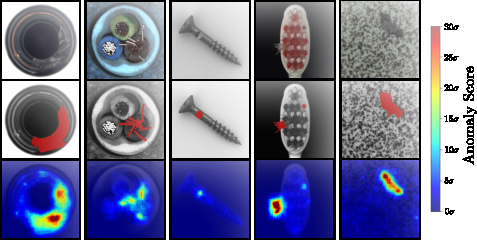
\includegraphics[width=\textwidth]{img/template-Goal.pdf}
  \end{columns}
\end{frame}


%%%%%%%%                      03 - Information                      %%%%%%%%
%---------------------------------------------------------------------------
% The purpose of the defence is to report on the project's status, not to hold a lecture on the given topic. Talk about what you have done and what your results are. Keep formal terms on your slides, be precise, define and refer.

% The presentation need not and, in fact, should not include:
% -- Explanation of algorithms used, etc. That belongs in a lecture about the topic. In your project presentation, it is typically enough just to list the used algorithms by name. Unknown algorithms can be explained a bit to clarify what they are, but don't explain them in detail. The goal is not for your audience to completely understand the algorithm and to be able to program it but to give them an idea of what you are working on and how you are doing it.
% -- Details of your system design. Again, your audience is not going to hack your system; they don't need detailed class structure, function names, file names, data formats, etc. Provide these things only to the extent that it helps the audience understand what you're are working on and how you are succeeding in it.

% HEROUT, Adam. Prezentování. Herout.net: Poznámky učitele, kouče, čtenáře. [online]. [cit. 2021-9-15]. Available at: https://www.herout.net/blog/category/prezentovani/
%---------------------------------------------------------------------------

% - Indicate what interesting problems you have solved in your thesis.
% - It should show that it is a thesis -- not just another project for a course -- so there is something non-trivial, interesting, and useful.
% - Rather have two or three slides that you show/explain in 20 seconds than trying to cram everything onto one slide.
% - It is good to put visual information on the slides: formulas, schemes, pictures, diagrams. Verbal information can be conveyed through your mouth. It is perfectly useless and annoying to have the same thing you are going to say in bullets on a slide.
% - The title of the slide, "Essential Information About the Solution", is very generic. In your actual slides, it would be much better to use a specific title on each of the slides, for example, "Neural Network Scheme for Big Nose Detection", "Design of an Infinite Automata", "Collected Dataset", etc.

\begin{frame}
  \frametitle{Essential Information About the Solution}
  \centering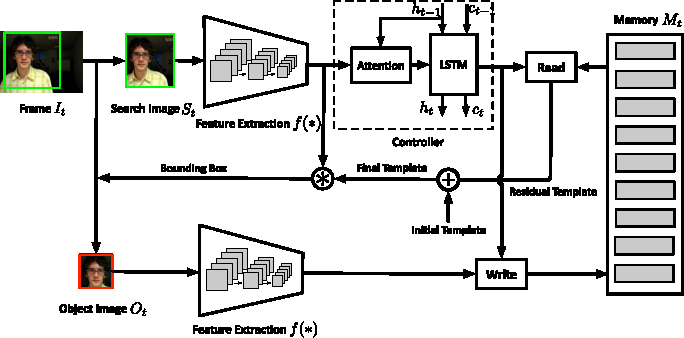
\includegraphics[width=0.8\textwidth]{img/template-Schema.pdf}
  \begin{equation}
      \mathbf{a}_t = \sum_{i=1}^{L}\alpha_{t,i}\mathbf{f}_{t,i}^{*}
  \end{equation}
  where $\alpha_{t,i}$ computes the \emph{softmax}:
  \begin{align}
      \alpha_{t,i} &= \frac{\exp(r_{t,i})}{\sum_{k=1}{L}\exp(r_{t,k})} 
      \\
      r_{t,i} &= W^a \tanh\left( W^h \mathbf{h}_{t-1} + W^f\mathbf{f}_{t,i}^{*} + b \right)
  \end{align}
\end{frame}

\begin{frame}\frametitle{Essential Information About the Solution}
  \makebox[\linewidth]{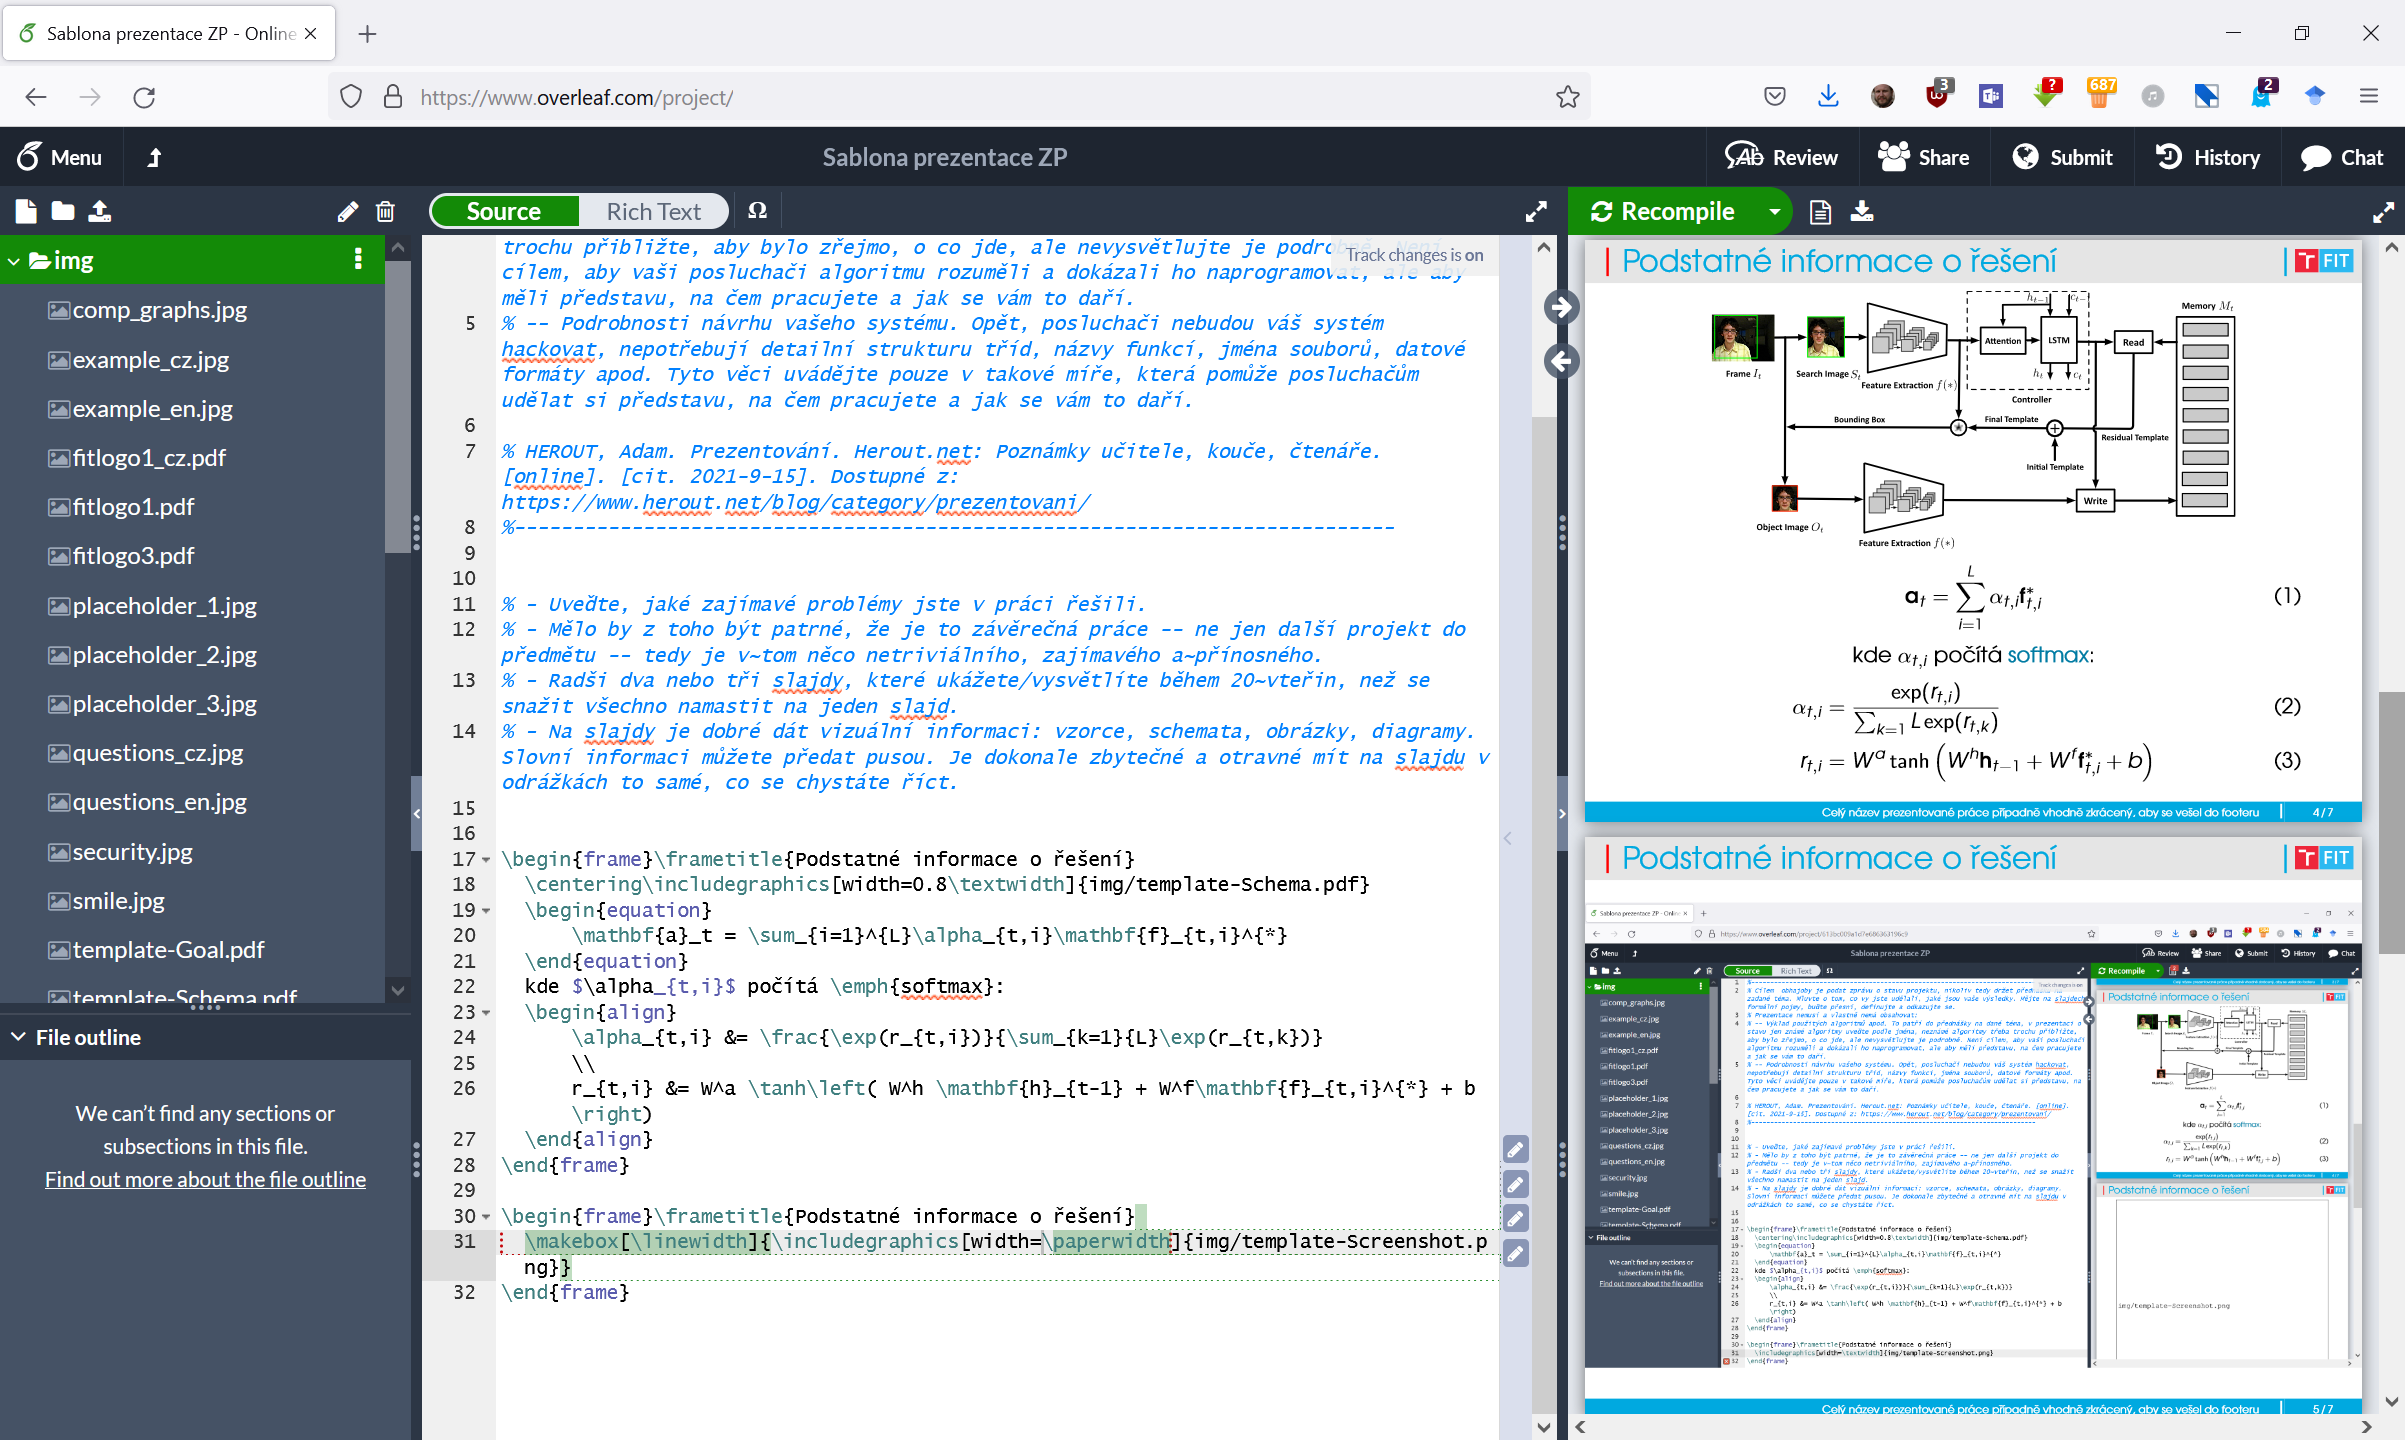
\includegraphics[width=\paperwidth]{img/template-Screenshot.png}}
\end{frame}


%%%%%%%%                        04 - Results                        %%%%%%%%
%---------------------------------------------------------------------------
% Summarise what results in you have achieved.
% Indicate how the functionality and correctness of the solution have been evaluated.
% Be specific: instead of "The application has been tested", say by whom and how it has been tested, and what the test results were.
% Instead of "The detector success rate is very good", say "The detector success rate is 93% mAP", or even better, show a table with a comparison against alternative solutions.
% If the evaluation consisted of two or three parts, splitting the content into two or three slides may be appropriate. When presenting, however, care should be taken to ensure that the time devoted to each slide is adequately short and that there is no time overrun.

\begin{frame}
  \frametitle{Experimental Results}
  \begin{columns}
  \column{0.4\textwidth}
    \begin{itemize}
      \item What has been \emph{done}
      \item Created dataset: \emph{105\,thousand} records
      \item Success Rate: \emph{103\,\%}
    \end{itemize}
    
  \column{0.6\textwidth}
    \centering
    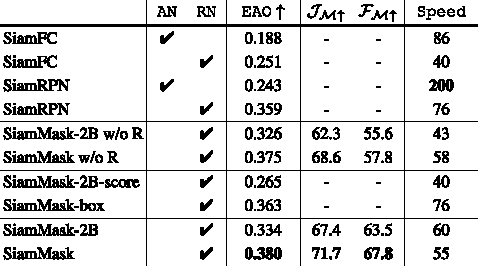
\includegraphics[width=0.8\textwidth]{img/template-ResultsTable.pdf}
    
    \bigskip
    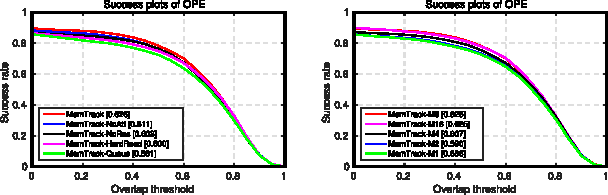
\includegraphics[width=\textwidth]{img/template-ResultsPlot.pdf}
    
  \end{columns}
\end{frame}


%%%%%%%%                        05 - Thanks                         %%%%%%%%
%---------------------------------------------------------------------------
% This slide should contain either one large or several smaller images arranged appropriately.
% Choose the best thing you want to show off - the committee will look at this slide the longest of all the slides.
% For this slide, thank the committee for attention (not necessarily by a huge text over the whole slide), and the committee will then have space to view the images as they listen to the reviews.
%---------------------------------------------------------------------------

% What is said at the end of the presentation is what the audience will consider when making subsequent decisions.

% HEROUT, Adam. Prezentování. Herout.net: Poznámky učitele, kouče, čtenáře. [online]. [cit. 2021-9-15]. Available at: https://www.herout.net/blog/category/prezentovani/
%---------------------------------------------------------------------------

\begin{frame}
  \frametitle{Thank You for Your Attention!}
  \centering
  \makebox[\textwidth]{
    \begin{tikzpicture}
      \node (screenshot) 
         {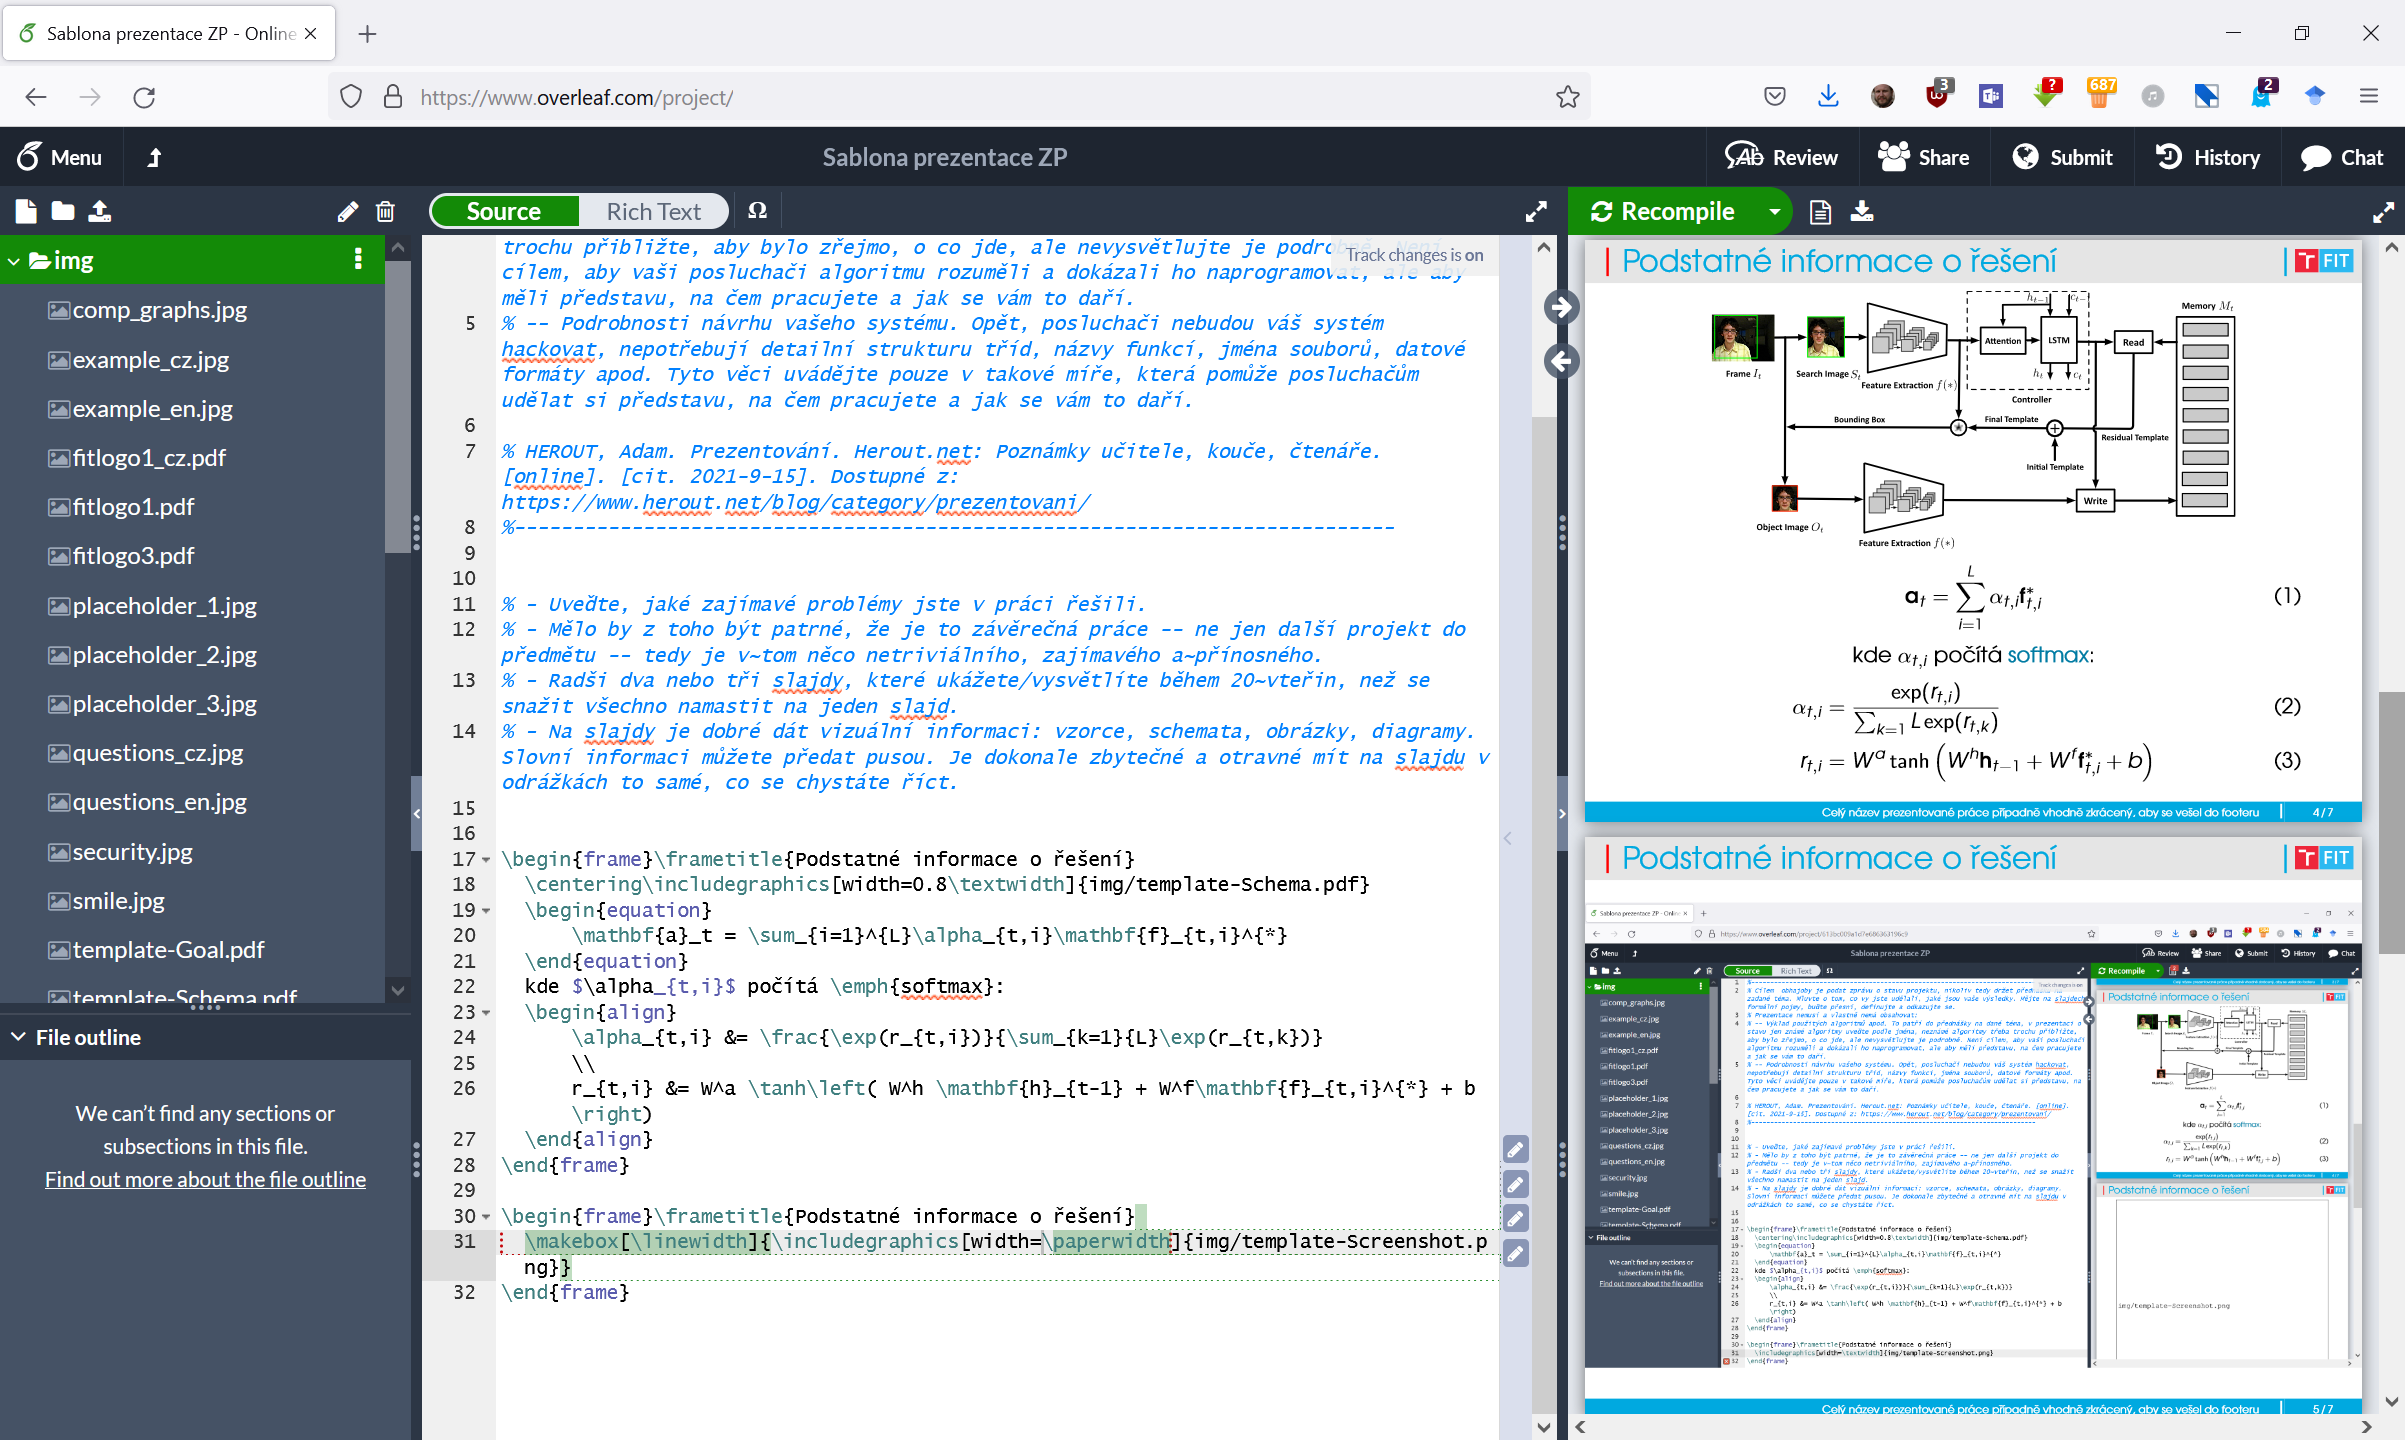
\includegraphics[width=0.6\paperwidth]{img/template-Screenshot.png}};
      \node (schema) at (screenshot.south east) [xshift=5em] [yshift=2.5ex]
         {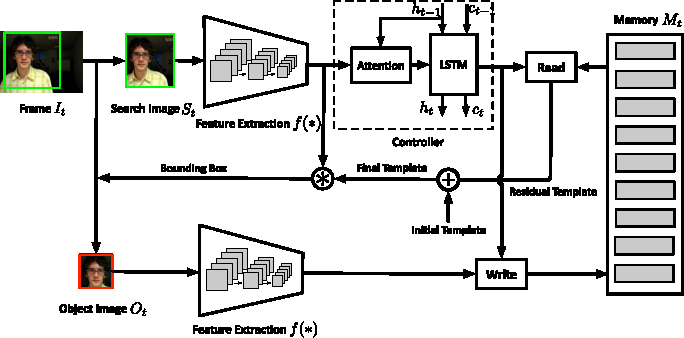
\includegraphics[width=0.45\paperwidth]{img/template-Schema.pdf}};
      \node (goal) at (screenshot.north east) [xshift=4em] [yshift=2ex]
         {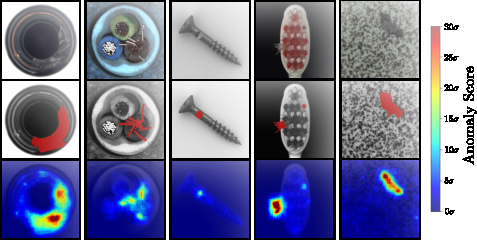
\includegraphics[width=0.5\paperwidth]{img/template-Goal.pdf}};
    \end{tikzpicture}
  }
\end{frame}


%%%%%%%%                       06 - Questions                       %%%%%%%%
%---------------------------------------------------------------------------
% At the State final examination:
%   1) The student presents his/her thesis, ends with "Thank you for your attention!"
%   2) The commission chairman organises what happens next: an extract from the reviews is read.
%   3) The student will answer the questions that the opponent has written in his/her review.
%   4) The student answers questions that come up in the room: from the committee members, but also from the guests.

% For point 3) above, it is helpful to have prepared slides:
%   A) They show the verbatim text of the opponent's question. The student reads it so that everyone knows it, and then answers it.
%   B) They will include visual aids to the answer.
%       a) Some answers to questions do not need visual support: the student simply says the answer, and everything is clear.
%       b) For other answers, it is wise to have a picture, a table, a graph, something that clearly shows the answer.

% The opponent's questions are not meant to be "topics for a lecture". If it can be answered in one sentence, it's better than fumbling around.
% Visual aids often help to answer succinctly, "The figure shows how I solve problem X." And that's it...

% If no visual information is needed for the questions, it is helpful to have them as bullets on a single slide.
% If there is more than one question and there are figures or graphs, it is advisable to have one slide for each question - the text of the question at the top, the visual material below.

\appendix{}
\begin{frame}
  \frametitle{Opponent's Questions}
  \begin{itemize}
    \item If there are multiple questions, more slides can be made.
    \item This slide should be an attachment that does not count towards the total number of slides.
    \item It is a good idea to transcribe the question here \emph{verbatim}, so that there is no doubt that there is no inaccurate paraphrasing.
  \end{itemize}
  \bigskip
  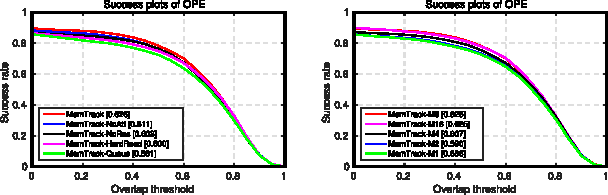
\includegraphics[width=\textwidth]{img/template-ResultsPlot.pdf}
\end{frame}  % Slajdy v angličtině / Slides in English
    \fi
\end{document}

%---------------------------------------------------------------------------
% Když připravujete prezentaci, rozmyslete, co budete říkat, pak rozmyslete, co by se k tomu hodilo mít promítnuté na plátně za vámi a pak podle toho připravte slajdy.

% Co je špatného na slajdech s mnoha písmenky
% -- Jejich nejčastější problém bývá, že slajd sděluje řečníkovu myšlenku. Po zobrazení slajdu si ho během několika vteřin všichni přečtou (a – chcete-li – během této doby řečníka neposlouchají). Potom řečník svoje publikum k smrti nudí tím, že jim říká, co už vědí – co se dočetli na slajdu.
% -- Stejné chyby se dopustí i ten, kdo svoji pointu sdělí stručným slajdem o čtyřech slovech, i ten, kdo svoji pointu proflákne roztomilým nákresíčkem.
% -- Slajd musí být hádanka – když se zobrazí, posluchač mu ještě moc nerozumí, neví, proč tu je. Pak, jak řečník mluví a vysvětluje, slajd dává víc a víc smysl, až dojde k prozření: „AHA, jasně!“

% Pár námětů na zamyšlení nad hotovými slajdy:
% -- Jsem se slajdy spokojený? S čím nejvíc, s čím nejmíň?
% -- Od kterých jednotlivých slajdů čekám, že posluchače nadchnou, nakloní na mou stranu?
% -- Kdyby mi někdo chtěl pokládat nepříjemné otázky – do kterého slajdu se bude strefovat?
% -- Které slajdy budou samy o sobě přitahovat pozornost posluchačů jen se objeví? Které slajdy budou nudit a budu pozornost ztrácet?
% -- Jaký „první dojem“ o vás sdělují první tři slajdy? „Tento student je …“ – co si komise doplní místo třech teček?

%---------------------------------------------------------------------------
% When preparing a presentation, think about what you're going to say, then think about what would be helpful to have projected on the screen behind you, and then prepare your slides accordingly.

% What's wrong with slides with many letters
% -- Their most common problem is that the slide communicates the speaker's idea. After the slide is shown, everyone reads it within seconds (and -- if you like -- doesn't listen to the speaker during that time). Then the speaker bores his audience to death by telling them what they already know - what they read on the slide.
% -- The same mistake is made by those who make their point with a brief four-word slide and those who make it with a cute sketch.
% -- The slide must be a riddle - when it appears, the listener doesn't understand it yet, doesn't know why it's there. Then, as the speaker talks and explains, the slide makes more and more sense when it comes to insight, "Ah, I get it!"

% Some ideas for thinking about the finished slides:
% -- Am I happy with the slides? With what the most, with what the least?
% -- Which individual slides do I expect to excite the audience, win them over to my side?
% -- If someone wanted to ask me uncomfortable questions - which slide would they aim at?
%  Which slides will attract the attention of the audience just by appearing? Which slides will be boring, and then I will lose attention?
% -- What "first impression" will you make with the first three slides? "This student is…" - what will the commission add instead of three dots?

% HEROUT, Adam. Prezentování. Herout.net: Poznámky učitele, kouče, čtenáře. [online]. [cit. 2021-9-15]. Dostupné z: https://www.herout.net/blog/category/prezentovani/
%---------------------------------------------------------------------------

% Obrázky / Pictures:
% -- STORIES. Freepik [online]. [cit. 2021-9-16]. Dostupné z: https://www.freepik.com/vectors/social-media
%---------------------------------------------------------------------------